\section{Project execution}
Projects at the eScience Center vary in duration from 3 months to 5 years, depending on the call through which they were
granted. In all call projects, the PM (with the help of Lead RSE) monitors progress of the project and involves
relevant stakeholders whenever necessary. The Lead RSE takes on a leading role during the execution phase of the
project life cycle. The Lead RSE ensures that the Project team meetings take place on a regular basis: the frequency
may vary with the size of the team, e.g. full team meetings once per month and meeting with only with the LA and/or LA
team once in two weeks.

\subsection{Project logging}
\label{sec:exec:log}
eScience project team members routinely log important project events and agreements. The project log is placed in the
Project portfolio (the Coordinators subfolder, see Appendix~\ref{app:folders}). The Lead RSE keeps the log up to
date (see example in Appendix~\ref{app:example-log}). The project log facilitates the information flow between
different stakeholders about project activities.

The following should be included in the project log:
\begin{itemize}
\item RSD project page URL
\item important meetings, including dates, links to slides and fully written agreements/decisions
\item infrastructure used and decisions regarding infrastructure
\item output/deliverables (their URLs, or this is registered as an output in RSD)
\item participation in workshops, external events, conferences related to the project (or this is registered as an output in
RSD)
\item changes to the project team
\item records on management plan updates
\item technology plan decisions and updates
\item results of (code) reviews of the project.
\end{itemize}

Links pointing to other documents (e.g., files in the Project portfolio, project output, repositories) should be used in
the project log to improve readability of the log and avoid duplicate information.

\subsection{Status update meetings}
\label{sec:exec:status}
The PM stays informed about the status of the project and communicates with the Lead RSE on a regular basis.

\begin{table}[h!]
\begin{booktabs}{colspec={|>{\bfseries}m{0.15\textwidth}|m{0.8\textwidth}|},row{even}={gray!20}}
    \toprule
    Scheduled: &  Once every 4-6 weeks \\[1.5ex]
    Stakeholders: & PM (organizer), Lead RSE, optionally: TL\footnote{The TL participation is mandatory for the techology-oriented projects.}, other RSEs. \\[1.5ex]
    Purpose: &  Status update on the project and discussion around project management. \\[1.5ex]
    Duration: & 30 min –- 1 hour \\[1.5ex]
    Location: & In-person meeting is default. \\[1.5ex]
    \bottomrule
\end{booktabs}
\end{table}

PM and Lead RSE discuss:

\begin{itemize}
\item project status (including any changes in a project workplan)
\item technological issues, with due consultation of TL, respective SIG, or other RSEs, if necessary
\item changes in technology plan, technological choices (Section~\ref{sec:init:techplan}), management plans (Section
\ref{sec:exec:mp}). For any of these changes, TL presence is required
\item synergies with other projects in the Center
\item issues related to the budget, communication, staffing, etc.
\item knowledge development and transfer, potential for software reuse, software sustainability.
\end{itemize}

The frequency and duration of these meetings are at the discretion of the PM and depend on factors such as the
experience of the Lead RSE and the size of the team and/or the project. 

In projects that have a stronger focus on technology (such as the eTEC, CIT projects), the TL is involved in these
meetings more frequently. For some projects, update meetings can be combined (e.g., for projects within the same Call)
or organized in the context of a larger meeting (such as a SIG on a relevant topic). Together with the Lead RSE, the PM
decides on the format of the status update meeting.


\subsection{Project team meetings}
To keep the entire project team informed on project progress, the Lead RSE together with the LA organizes a periodical
project meeting. The frequency and format depend on the complexity of the project and size of the project team.

\begin{table}[h!]
\begin{booktabs}{colspec={|>{\bfseries}m{0.15\textwidth}|m{0.8\textwidth}|},row{even}={gray!20}}
    \toprule
    Scheduled: &  Once every 2-6 weeks \\[1.5ex]
    Stakeholders: & Lead RSE or LA (organizer), LA (chair), RSEs and other project team members from the LA side. \\[1.5ex]
    Purpose: &  Progress update on the project by all team members. \\[1.5ex]
    Duration: & 30 min –- 1 hour \\[1.5ex]
    Location: & In-person meeting is default. \\[1.5ex]
    \bottomrule
\end{booktabs}
\end{table}

The agenda of this meeting should include:
\begin{itemize}
\item status update from all stakeholders
\item discussion of scientific progress
\item discussion of technological progress, issues and choices
\item alignment of project progress with the project workplan, and adjustment of the latter, if necessary.
\end{itemize}

\subsection{Writing hours and managing project budget}
\label{sec:exec:budget}
The PM and Lead RSE must have a firm grasp of the project budget and the project duration. This information is in the
Awarding letter, the proposal and Exact.

The project execution phase roughly consists of three parts: exploration, implementation, sustaining and dissemination.
For the call projects, the rough breakdown of work vs budget is as follows: 25\% of the time and budget goes to
exploration (including learning), 50\% of the budget is to be spend on development, and 25\% is for usage,
sustainability and dissemination activities. In addition, the budget of a project should be spent at a constant rate
during the runtime of the project. Lead RSE must discuss with the PM if project execution deviates from this plan.

\begin{figure}[!h]
    \centering
    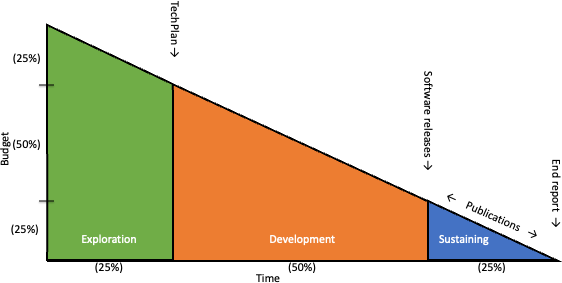
\includegraphics[scale=0.45]{img/budget-stages.png}
    %\caption{Project's budget breakdown}
    %\label{fig:project-budget}
\end{figure}

The eScience project team (including PM and RSEs) must submit their project hours in Exact by the end of each month. For
regular call projects, RSEs can write hours on awarded projects as soon as they are active in Exact, which in general
happens within a month of the project being granted. The PM writes management hours on the project budget.

Project hours are managed by different parties with different responsibilities:
\let\myhcolw\relax 
\newlength{\myhcolw}
\setlength{\myhcolw}{0.4\textwidth}
\begin{table}[!h]
\renewcommand{\arraystretch}{1.5}
\begin{booktabs}{colspec={|p{0.12\textwidth}|p{0.4\textwidth}|p\myhcolw|},row{even}={gray!20}}
    \toprule
    \textbf{Stakeholder} &  \textbf{Responsibilities} & \textbf{More info} \\\toprule
    PM & 
    \begin{minipage}[t]{\myhcolw}
    \begin{itemize}\itemsep0em
        \item checks and approves the hours submitted in Exact for the projects for which they are accountable before the 5th workday of the next month
        \item provide monthly hour status to the Lead RSE 
        \item checks and signals to F\&C if there is an issue (for example, if project budget is incorrect)
        \item informs F\&C about project budget changes made by PM or DT
    \end{itemize} 
      \end{minipage}
    & \\\midrule
    Lead RSE &     
    \begin{minipage}[t]{\myhcolw}
    \begin{itemize}\itemsep0em
        \item monitors project hour expenditure and signals deviation from the workplan to the PM
    \end{itemize} 
      \end{minipage}
    &  Asks PM for hours status in Exact, or checks monthly budget status via Ganttic  \\\midrule
    F\&C &
    \begin{minipage}[t]{\myhcolw}
    \begin{itemize}\itemsep0em
        \item maintains accurate budget information 
        \item monitors and processes approved project hours
        \item makes financial information available to the budget holders (including PMs) each month 
        \item automatically puts read-only status on the project when project hours are depleted/exceeded early
    \end{itemize} 
      \end{minipage}  
    & All budget changes require a PM and DT decision. \\\midrule
    DoT & 
    \begin{minipage}[t]{\myhcolw}
    \begin{itemize}\itemsep0em
        \item monitors and approves software sustainability hours 
    \end{itemize} 
      \end{minipage}
    & There is a separate protocol on handling software sustainability. \\
    \bottomrule
\end{booktabs}
\end{table}

Hours must be submitted and approved on time, preferably on a weekly basis. All data must be entered no later than one
working week following the end of the month.

In some projects, the LA and RSEs are free to spend the awarded hours faster than originally planned. However, the Lead
RSE is responsible for results being delivered on time for the project and not exceeding the budget, and for timely
informing the PM. If a project budget is fully spent ahead of its schedule, the PM asks F\&C to restrict writing on the
project budget only to the PM.

It is possible to travel for a project, however RSEs must ask approval of their line managers (a respective SH) before
committing to an event requiring travel and fill out a travel form. See the Intranet for more information.

For \textbf{external projects}, the rules on writing hours differ from regular call projects. Only RSEs and the PM
working on the project are allowed to write hours on the project budget. Moreover, for some projects (e.g., Horizon
Europe projects) only direct contributions to the project are allowed; other non-project related activities such as
time spent on a SIG cannot be declared on these projects. The Lead RSE and PM are aware of restrictions related to
their project.

\subsection{Workshops}
\label{sec:exec:workshops}

Some call projects require the LA to organize workshops. These workshops aim at fostering research communities around
the software we develop on projects. A focus of a workshop could be, for instance, the early adoption of software
requirements suggested by potential users, the addition and expansion of new features, or the linking of the exiting
tool to a wider or more mature community. Based on the call text, the PM determines whether one of more workshops must
be organized. There are two types of workshops, namely,
\begin{itemize}
\item organised by the LA
\item organized by the Lorentz Center.
\end{itemize}

For workshops organized by the LA themselves, the LA writes and submits the workshop plan(s) to the PM (cf.~\cite{proj-templates} 
for the templates) in a timely manner. The plans need to be approved by the PD and F\&C. The
Lead RSE is expected to contribute to the workshop and its organization. A CM can advise the LA (via the Lead RSE) on
supporting the engagement and growth of relevant communities around the software; a CM is involved in the introductory
part of the workshop, including an opportunity to address participants. F\&C supports the PM team with respect to
reimbursement of the costs and records that a workshop took place. Detailed procedure of workshops approval is
described in Appendix~\ref{app:workshops}.

For workshops organised by the Lorentz Center, the LA must apply through the Lorentz Center webpage\footnote{The
procedure is described in the eScience - Lorentz Center Agreement and Annexes {\textcolor{red}(add the link when signed)}.}.

The LA has the leading role in the application. The Lead RSE takes an advisory role in the writing and design of the
workshop proposal and is expected to actively participate during the workshop event. The PM must ensure enough hours
are allocated for the Lead RSE (or RSE from the project team) to help the LA with the proposal and attend the workshop,
if they want to take an active role.

These workshops differ from the eScience-Lorentz Center Competition workshops that are funded by both the eScience and
the Lorentz Center. Besides co-funding workshop expenses, the eScience Center supports such a workshop with an
additional in-kind contribution. The role of the eScience RSEs is described in the awarded proposals. The project
initiation and assignment of the eScience project team proceeds similar to other type of project. The eScience team
clarifies with the organizers the planning and outcome of the workshop (e.g. research paper, white paper, software
release, consortium creation for a grant application, etc.). The Lead RSE has a pivotal role in the preparation and
delivery of the workshop, and, possibly, in post-workshop stage to publish any outcome drafted during the event. 

\subsection{Data and Software Management Plans}
\label{sec:exec:mp}
For some projects, Data and Software Management plans (DMP~\cite{dmp-guide} and SMP~\cite{smp-guide}, respectively) provide details regarding the
maintenance of the data and software output of the project.

Depending on the call, the LA must provide a fully worked out SMP and DMP within the first 6 months of the project. The
Lead RSE can assist the LA and their team in drafting the DMP. The LA submits the DMP to the PM, who asks a TL for
review and approval. For call projects since 2021, an SMP is a part of the proposal itself. 


The LA maintains these plans and communicates any changes to the PM and TL via the Lead RSE. If needed, the PM requests
an update. The Lead RSE can help the LA to update the plans.


\subsection{Knowledge transfer}

To increase visibility of the project and its results, the project team (including RSEs, PM, TL), Communications, CMs,
share knowledge and outcomes both inside and outside of the organization. The Lead RSE ensures that
\begin{itemize}
\item information on project results is properly shared with Communications, CMs and relevant SH in a timely manner;
\item project and software pages on the RSD are properly updated; and
\item specific requests to facilitate project visibility are sent to Communications by RSEs.
\end{itemize}

Moreover, PMs, Lead RSEs and TLs work together to spot opportunities for cross project collaboration (e.g., by reusing
software or knowledge in these projects or as a new reusability project, read more in Section~\ref{sec:opportunities:ss}).



\subsubsection{Output management}
\label{sec:exec:output}
Projects deliverables include output such as research articles, presentations, invited talks, posters, tutorials,
datasets, blog posts, white papers and workshops but also more software-oriented output types such as software or code
releases, dedicated software publications, software demonstrators, software videos, tutorials and training material
around software.

RSEs strive to apply FAIR principles~\cite{fair-principles,FAIR4RS} to all project deliverables. Therefore, all project deliverables should have

\begin{itemize}
\item concept DOIs (obtained from the publisher or created by uploading to Zenodo, arXiv, DANS or similar open-access
archives);
\item acknowledge the eScience Center project grant; and
\item listed RSEs working on the project as (co-)authors.
\end{itemize}

To formally record results and facilitate knowledge transfer, RSEs must make all project output available in the
relevant systems, online locations and databases:

TODO

In terms of project output, the PM expects the project team to follow the plan on deliverables; project deliverables are
described in the proposal and workplan. RSEs contribute to the publications and software/data releases.

Open access publications and open software are a requirement for all call projects; PM and Lead RSE keep the LA informed
on this matter, if necessary. The funds for open access publication fees are internally budgeted in the call budget by
F\&C (with the approval of the PD every year). The Lead RSE and PM consult F\&C regarding payments for an open access
publication.

For \textbf{external projects} the expected deliverables are also part of the formal project documents (proposal,
contract, etc. The Lead RSE is expected to keep the PM informed of the status of deliverables throughout the project.


\subsubsection{Outreach}
\label{sec:exec:outreach}
The Lead RSE stimulates and promotes the visibility of the project through project demonstrators, presentations, and
other means. All RSEs are expected to communicate about the project and its deliverables externally, as
described in Section~\ref{sec:exec:output}. Communications advises and supports the project team to
highlight projects through various communications channels, including but not limited to news items, social media
posts, videos and interviewing team members about relevant scientific output and impact obtained as a result of the
research software applied or developed in the project). The Lead RSE (or in rare occasion the PM) contacts
Communications with relevant information. 

Blog posts are an optional but highly recommended output of the projects. They can be authored by any member of the
project team, from LA to RSE. Topics for a project's blog post can vary greatly. Examples
include, but are not limited to,
\begin{itemize}
\item a simplified version of (parts of) the research, or 
\item a tutorial about a skill or technology a member of the team has learned during the project
\item a communication about workshops, publications, releases or other type of project output.
\end{itemize}

RSEs engage in activities to inform colleagues about the project and the results (e.g., technology plan, milestones,
code releases), including presentations at SIGs. For internal and external events, each RSE should prepare a
three-slide presentation or a pitch~\cite{three:slides} 
regularly update it. The Lead RSE is responsible for ensuring a presentation in the form of a demonstrator (e.g., of the
software developed in the project) is available after the first major release of the software.


The LA and their team are encouraged to participate in relevant Digital Skills Workshops~\cite{digital-skills} from the eScience Center. Furthermore, if the LA and their team
require a project-specific training workshop, the Lead RSE involves
\begin{itemize}
\item workshop coordination (via CMs) who can advise the eScience project team with workshop organization and the development
of new training material. If applicable, the payment for the overall organization (either through or on top of the
project budget) is handled by F\&C; and
\item the PM to discuss the RSE hours spent on organizing the training. If necessary, the PM contacts F\&C for a consult.
\end{itemize}

Again, for \textbf{external projects} separate agreements may exist with the project consortium on how to communicate
results of the project (for example, Non-Disclosure Agreement or NDA). The Lead RSE and PM consult these agreements at
the start of project to know what can be communicated and what not.

\subsection{Code quality and sustainability checks}
Taking care of software quality and sustainability is integral to the code development process cycle at the eScience
Center. All RSEs must follow our guide and best practices~\cite{guide-nlesc} for software development. Code should be made
as generic and reusable as possible from the start.

\subsubsection{Code development}
\label{sec:exec:code}
At the initial stage of code development in the project, the Lead RSE together with RSEs:

\begin{itemize}
\item set up a GitHub organization for the project, following the eScience Center Guide and the Turing Way~\cite{the_turing_way-2023}
\item add the URL of this organization to the RSD project page.
\end{itemize}

RSEs must always ask at least one project team member, relevant SIG member or other RSE at the eScience Center to
review, comment and approve pull requests in the project codebase.

\subsubsection{Code review}
As part of the annual review (see Section~\ref{sec:exec:annual}), a code review is organized by the Lead RSE. Depending
on the project it could take the form of a reusabilithon\footnote{The term coined by the Software Sustainability SIG.
It refers to the 2-3 hours session with a group of RSEs to check usability of a software, give feedback to the
developers and to come up with recommendations to improve the software (re-)usability.}, a review of code on GitHub, or
something else entirely (format to be approved by TL). The reviewers for this process are typically other RSEs at the
eScience Center.


The goal is to review software of the project for:
\begin{itemize}
\item its usability (reproducing steps of installations, and running it on a machine/laptop)
\item overall software quality and suitability
\item whenever appropriate, correctness of code
\item adherence to the technology plan (Section~\ref{sec:init:techplan})
\item adherence to eScience Center best practices
\item opportunities for reuse of software in other projects
\item correct inclusion in output systems (Section~\ref{sec:exec:output}).
\end{itemize}

Reviewers make written suggestions for improvements, and flag major issues encountered. These issues serve as input for
the TL for the formal annual review meeting (see Section~\ref{sec:exec:annual}). These notes are stored in the project log. 

\subsection{Annual project review meeting}
\label{sec:exec:annual}
For all call projects lasting longer than one year, the PM organizes annual reviews. The details are described in the
terms and conditions document~\cite{nlesc-terms}. For the projects with the
duration of exactly one year, organizing a review meeting is at the discretion of the PM (in consultation with TL and
Lead RSE). 

A standard part of every review is a discussion and list of actions on how the results of the project will be made
reusable and sustainable (as described in the DMP and SMP), how the collaboration is going and possibilities for
follow-ups to projects.


\let\myhcolw\relax % let \myhcolw to \relax to be reused later
\newlength{\myhcolw}
\setlength{\myhcolw}{0.75\textwidth}

\begin{table}[!h]
\begin{booktabs}{colspec={|>{\bfseries}m{0.2\textwidth}|m{\myhcolw}|},row{even}={gray!20}}
    \toprule
    Scheduled: &  Yearly \\[1.5ex]
    Stakeholders: & PM (chair), Lead RSE, LA, TL, optional: other project team members, SH \\[1.5ex]
    Purpose: &  %
    \begin{minipage}[t]{\myhcolw}
    \begin{itemize}\itemsep0em
        \item to ensure that the project is still on track
        \item to discuss any persistent issues to ensure optimal collaboration between project team
        \item to explore opportunities beyond the project  
    \end{itemize} 
      \end{minipage}
    \\[1.5ex]
    Outcomes/Actions: & List of agreements, action points, advises (from the PM and the TL) for project team members on future steps. \\[1.5ex]
    Duration: &  Max 1.5 hours \\[1.5ex]
    Location: &  At the eScience Center or the project location\footnotemark{} \\[1.5ex]
    \bottomrule
\end{booktabs}
\end{table}
\footnotetext{Mandatory participants of a meeting be present in-person at the office, while all optional participants
can also participate via video conferencing if they prefer.}



The agenda of this meeting is:
\begin{itemize}
\item Introduction by eScience Center (round of introductions and purpose of meeting)
\item project overview and deliverables so far
\begin{itemize}
\item status of the scientific goal(s) by the LA and their team
\item status of the output (e.g., publications, software, datasets, methods, documentation) by the project team
\end{itemize}
\item status of the collaboration (including admin status of hours, bottlenecks)
\item use of digital infrastructure and support of SURF (if applicable)
\item next steps
\item opportunities beyond the project.
\end{itemize}

The goals of the meeting are to:
\begin{itemize}
\item review the progress of the project in comparison to the original workplan (are we on track?)
\item discuss research results and their novelty and current deliverables of the project
\item discuss status and update the management plans, if necessary
\item discuss strategies to expose project results to a broader community
\item discuss strategies and actions to ensure the reuse and sustainability of the software
\item identify bottlenecks and areas for improvement to ensure efficient work of the project team
\item report financial status of the project (RSE hours left)
\item brainstorm on further collaboration and funding options, if relevant
\item brainstorm on the potential for cross project collaboration.
\end{itemize}

For \textbf{external projects}, review meetings are usually organized as part of the project process. Whether or not (a
lightweight version of) our internal review procedure is needed for a project is determined by the PM, in consultation
with the Lead RSE.


\subsubsection{Review meeting preparation}
\begin{table}[h!]
  \renewcommand{\arraystretch}{1.5}
\begin{booktabs}{colspec={|>{\bfseries}m{0.3\textwidth}|m{0.6\textwidth}|},row{even}={gray!20}}
    \toprule
     &  \textbf{Stakeholder} \\[1.5ex]\toprule
    Prepared by: & LA and Lead RSE of the project. Other stakeholders of the project can contribute. \\[1.5ex]
    Reviewed by: &  PM accountable for project, TL accountable for technology. \\[1.5ex]
    Target audience: & PMs, TLs, SHs and RSEs. \\[1.5ex]
    \bottomrule
\end{booktabs}
\end{table}

The PM sends the LA team the standard review meeting presentation template~\cite{proj-templates}, updating the slide on RSE hour status. This
template provides a list of the important points to be discussed. LA and Lead RSE collaboratively prepare the slides.
In particular, 
\begin{itemize}
\item the LA adds 3-5 slides (can be separate from the template) to report concisely on the extent to which the research
objectives of the project have been met. The LA is not expected to present the content of published papers or the
original workplan or proposal;
\item the Lead RSE prepares 1-2 slides on a status of the current technology plan and software, datasets, methods or/and documentation, 
  and remarks on reusability, adoptability and sustainability of the software;
\item the LA and Lead RSE compile the list of project deliverables. If applicable, the LA reports on the workshops;
\item the Lead RSE compiles the technology status report (see Section~\ref{sec:exec:tech}) based on the input from LA and
the rest of the project team, and provides it to the TL;
\item the LA and Lead RSE point out any scientific or technological bottlenecks, e.g., approaches that did not work, data that
was not collected, or any other reasons for delays in the workplan. To this end, the LA and Lead RSE comment if the
project is on track or whether the planning needs to be revised;
\item the PM reports on the financial status of the project (the number of hours already spent); and
\item the entire project team is invited to comment on how the collaboration is going, in terms of interaction between the
team members and suggestion for improvements, if there are any issues.
\end{itemize}


The Lead RSE:
\begin{itemize}
\item requests other project team members to contribute to the slides, wherever appropriate, and technology status report;
\item meets with CM before the review meeting to draft the technology status report, and together with TLs to draft the rest
of the report.
\item coordinates with the entire project team to finish the preparation of the presentation at least 2 working days before
the review meeting;
\item ensures that output is correctly registered in systems described in the output management (Section~\ref{sec:exec:output}) 
  and all missing URLs and DOIs are added to the slides;
\item uploads the slides to the project portfolio (into the Reviews subfolder, see Appendix~\ref{app:folders}.); and
\item informs PM and TL that slides are ready and are in the project portfolio.
\end{itemize}

\subsubsection{Technology status report}
\label{sec:exec:tech}
Prior to the annual review meeting, the PM asks Lead RSE to fill in the technology status report. This is a document
containing an overview of the technical development of the project such as project RSD page with its deliverables, URLs
to project plans, and information on quality and community involvement. The information provided by the Lead RSE (in
collaboration with the project team) in this report serves as input for the TL at the project review meeting.

Two weeks prior to the review meeting, the TL should receive from the Lead RSE the filled-out
form. Based on the final report the TL performs a code review or software health check, and ensures that the review
results are shared with the eScience project team before the annual meeting. The Lead RSE, the TL and the PM can meet
additionally to discuss the status report and/or the results prior to the annual review meeting.

The report and the review are archived by the TL in the project portfolio folder.

\subsubsection{At the review meeting}
The time breakdown of the meeting agenda is follows:
\begin{itemize}
\item presentation by the LA (max. 20 min)
\item presentation by the Lead RSE (max. 20 min), including a description of RSE roles and project deliverables.
\item discussion (max. 40 min)
\item summary, action points and conclusions.
\end{itemize}

The PM chairs the meeting, acting as a reviewer together with the TL. The TL raises possible issues related to
technology and software. Other invited stakeholders can comment and contribute to the discussions. The PM and TL
comment on the status of the deliverables:

\begin{itemize}
\item have the objectives outlined in the proposal been sufficiently addressed? (PM)
\item does the project follow the workplan in terms of deliverables? (PM)
\item has the output been registered according to the rules of output management (Section~\ref{sec:exec:output})? (PM, TL)
\item does all project output have publications (including software and data papers)? (PM)
\item are there any issues flagged during the code review that needs to be discussed with the project team? (TL)
\item does the project team sufficiently engage and align with relevant communities (e.g., via the workshops)? (PM)
\item does the project adhere to the technology plan, SMP and DMP? (TL)
\end{itemize}

The eScience project team comments on any further possibilities for reusability, adoptability and sustainability of the
software, and the project team comments on possible collaborations beyond the project.

The PM updates the slides with action points, agreements and plans (with the project partners agreement). The PM logs
the meeting in the project log.

\subsubsection{After the review meeting}
PM shares the updated slide deck with the project team members to check the agreements written down. PM ensures that the
final version of the presentation(s) uploaded to the project portfolio is correct.

\subsection{Reporting}
For call projects the annual review meeting and end report serve as formal progress reports.

\textbf{External projects} may require periodic reporting to the consortium on progress according to the workplan,
including deliverables. The PM and Lead RSE consult the Consortium/Collaboration Agreement, the contract and the
proposed workplan and involve F\&C for the financial part of the report. Normally, the external project coordinator
(e.g., EU project coordinator, NWO programme officer) signals the deadline of a deliverable or report. The Lead RSE
contributes to the report on project activities required to be done by the eScience Center, and the PM checks the
document. The PM asks F\&C to check or fill in the financial part of the report, signed by the DoO if necessary. Once
the final version is ready, the PM sends it to the external project coordinator (via EU portal done by F\&C) and
archives this report in the project portfolio.

\subsection{Conflict resolution and complaint procedure}
The eScience Center follows the Code of Conduct as outlined in the Personnel Policy (cf.~\cite{cao-intranet} for the details).

All conflicts on projects involving the eScience Center RSEs and the LA and their team should be resolved using the
following four-step process:

\begin{enumerate}
\item When problems arise in a project, the Lead RSE is expected to resolve problems in consultation with the LA. If needed,
the PM can be asked to join in discussions on finding the best course of action;
\item Both RSEs and LA can escalate issues related to the project to the PM (preferably, via the Lead RSE). The PM organizes a
meeting to discuss the problem and tries to resolve it;
\item If the problem remains unsolved, the RSEs or the LA can escalate it to the PD by sending a letter summarizing the
situation to the accountable PM, who will forward it to the PD; and
\item The PD can escalate the problem to the DT.
\end{enumerate}

If the problem is with the PM, RSEs can escalate to their manager (SH).

The eScience Center also has an external confidential advisor ('Vertrouwenspersoon') who can be contacted anonymously. See the Personnel
Policy for details.

Resolving conflicts may result in changes to the project, such as changes in staffing or changes described in Section~\ref{sec:init:vacancy}.

\subsection{Non-RSE Consultants}
\label{sec:exec:consult}
Certain issues will require that the project team consults with other persons inside the eScience Center. The following
situations require the team member to notify the PM, any actions may be delegated to any eScience team member:

\begin{itemize}
\item For project related GDPR issues, or personal identifiable data, consultation with the GDPR contact person is
obligatory. For contacts, cf. GDPR section on the Intranet~\cite{proj-intranet}. 
\item For issues related to software or data accessibility and quality, contact the TL.
\item For issues related to scientific integrity, contact the scientific integrity officer (cf. the Intranet page~\cite{proj-intranet}).
\item For issues related to SURF (use of their infrastructure or need of advisor), contact SURF liaisons. For
contacts, see the intranet page~\cite{access-infra}.
\item For issues around sustainability, contact the TL and CMs.
\item For IP and licensing issues, contact the DoT.
\item For legal matters, contact the DoO (cf. Section~\ref{sec:init:legal}).
\item For external opportunities, contact PD (cf. Section \ref{sec:opportunities:external-funding}).
\end{itemize}

\subsection{Changes to the project}
\label{sec:exec:changes}
During the project life cycle, the workplan may change substantially:

\begin{itemize}
\item New deliverables because of additional funding
\item New workplan because of changes in the research goal and/or in the technology used
\item Timeline, leading to a different end date.
\end{itemize}

Any of these changes needs explicit approval from the PM team or the DT.

\begin{table}[h!]
\begin{booktabs}{colspec={|m{0.65\textwidth}|m{0.3\textwidth}|},row{even}={gray!20}}
    \toprule
     \textbf{Type of request} &  \textbf{Decided by:} \\[1.5ex]
    Budget requests within the PM mandate (see Appendix~\ref{app:pm-mandate}.) & PM team \\[1.5ex]
    All requests regarding budget changes outside the PM mandate &  DT (via PD) \\[1.5ex]
    Early termination & DT (and DT informs the Board) \\[1.5ex]
    \bottomrule
\end{booktabs}
\end{table}


For \textbf{external projects} changes to a project must be handled as described in the formal documents for this
project (e.g., grant agreement, consortium agreement). If it is within the PM mandate, the PM discusses with the PM
team any extensions required for the project. Otherwise, the decision is made by the DT. The PM informs the external
funder or consortium of the decision.

\subsubsection{Proposal changes request}
The LA must submit a formal request to the PM team (by email via the PM, in PDF format, signed) containing:

\begin{itemize}
\item project title and project number
\item requested change (e.g., time/dates, RSE hours, scientific goal) and motivation for this change
\item conditions such as deliverables: 
\begin{itemize}
\item If there are new deliverables, what are those and what is the new planning? 
\item If there are no new deliverables, that should be stated explicitly.
\end{itemize}
\item any motivated budget change, such as 
\begin{itemize}
\item LA wants to increase their involvement 
\item change in research personnel (if applicable in the case of older projects)
\item transfer from hardware costs to RSE contribution or PYR for research personnel on the LA side (or vice versa) (if
applicable in the case of older projects)
\item any in-kind to cash change, or vice versa (including requests with the extra cash budget from the LA).
\end{itemize}
\item any prior or planned inactivity on the project, such as
\begin{itemize}
\item shortage of personnel on the LA side due to e.g. maternity leave, sick leave, hiring delays (for example, a PhD student
or a postdoc needs to be hired but there is a concise timeline on the hiring procedure)
\item unavailability of RSEs 
\item additional data that needs to be collected.
\end{itemize}
\item any delay with the start date.
\end{itemize}


\subsubsection{Processing the changes request and decision}
Upon receipt of the request, the PM assesses if the request should be granted based on considerations such as 
\begin{itemize}
\item whether the new objective is scientifically promising or technologically interesting? (if applicable)
\item collaboration status with the LA;
\item prior problems regarding the project;
\item the benefit of continuing the project for the eScience Center (e.g., good wrap up of the collaboration, this leads to
another funding opportunity together); and/ or
\item availability of RSEs with relevant expertise to work on it.
\end{itemize}

The PM can consult with RSEs and the TL on whether the new planning is feasible. In case of additional funding, the DT
(via the PD) will decide, after a budget calculation by the F\&C and approval by the DoO. Otherwise, the PM puts the
request on the agenda for the next PM meeting, containing: 
\begin{itemize}
\item the motivated request (uploaded to the project portfolio, the subfolder titled Coordinators (see Appendix~\ref{app:folders} for more details on the folder structure.)
\item the recommended action
\item the prepared decision on the PM meeting agenda (uploaded to the project portfolio, the subfolder titled Coordinators).
\end{itemize}

The PM team may request more information from the LA via the PM (and thus postpone the decision on the request). The LA
can provide the new information via an additional PDF signed letter or as amendment to the original letter.

After the final decision, the PM notes the official decision in the decision document. If the request is not approved,
the PM communicates this to the LA. If the request is approved, the PM
\begin{itemize}
\item communicates with F\&C, which finalizes the extension (changes in Exact, the extension letter for the LA);
\item double checks if budget and hours in Exact are still correct;
\item updates planning and adjusts staffing, if necessary;
\item ensures website and RSD are updated (e.g., if dates or affiliation changed); and
\item communicates the extension to the project team.
\end{itemize}


If the request involves a DT decision, the PM submits a request formally through the PD.

\subsubsection{Early project termination}
Early project termination can be
\begin{itemize}
\item agreed on by mutual consent;
\item initiated by the LA; and/ or
\item initiated by the eScience Center.
\end{itemize}

In the first and the second case, the PM submits a letter (written together with and signed by the LA) explaining the
situation to the DT. The letter should contain (a proposal for) an agreement on how to handle all the remaining
resources of the project (RSE hours, cash contribution, FTE commitment for LA, workshops, software sustainability
budget, etc.). 

The PM can request the termination of a project if the conditions and agreements in the Awarding letter and Bijzondere
voorwaarden have been violated by the LA or the project partners. The PM submits the letter to the DT (via the PD
explaining the situation). If the DT approves the termination, the PM communicates this decision to F\&C, which
finalizes the process (by making changes in Exact and preparing a termination letter).

\subsection{Opportunities beyond the project}
\label{sec:opportunities}
A project team can explore different opportunities for ideas that stem from the project that go beyond its scope and/or
budget. Appendix \ref{app:pm-role} summarizes the role of PM in such projects. The PM discusses these opportunities with the project
team during the review meeting.


\subsubsection{Increasing reusability (in this document called software sustainability)}
\label{sec:opportunities:ss}
For some projects, or entire calls, specific budget is available for software sustainability. Until 2020, each
individual project was assigned a so-called Generalization budget (“Generalisatie”), for generalization and reuse of
project results. Since 2020, however, this budget is no longer assigned per project, but for the entire programme/call.
The PM and the Lead RSE check the corresponding call text and the awarding letter of the project to determine If the
software sustainability budget is available.

The PM signals potential for reusability to the TL. The TL discusses this opportunity with the Lead RSE and if
necessary, the TL team. If RSEs have an idea and are interested to work on a project funded by this budget, they may
contact TLs or DoT for more information. The process follows the SS protocol~\cite{ss-intranet}.

\subsubsection{Knowledge and Development}
\label{sec:opportunities:kd}
For the development of broad and deep knowledge on digital technologies and their application, RSEs can apply for
so-called Knowledge and Development (KD) project. The process is described by the KD protocol~\cite{kd-intranet}.

\subsubsection{External funding}
\label{sec:opportunities:external-funding}
The project team may decide to pursue other funding opportunities. The eScience Center encourages RSEs to pursue
external funding opportunities to promote the organization profile as research organization. PD oversees the
Acquisition activities and the process. The relevant information is available via Intranet~\cite{external-intranet}.


\subsubsection{Fellowship}
\label{sec:opportunities:fellowship}
To stimulate community engagement lasting longer than project lifetime, the eScience Center funds annual Fellowship
Program~\cite{fellowship-intranet}. The eScience project team is not eligible for this program, however, the LA and their team are.